Global and local thresholding



\begin{figure}[ht] 
    \begin{subfigure}[b]{0.5\linewidth}
      \centering
      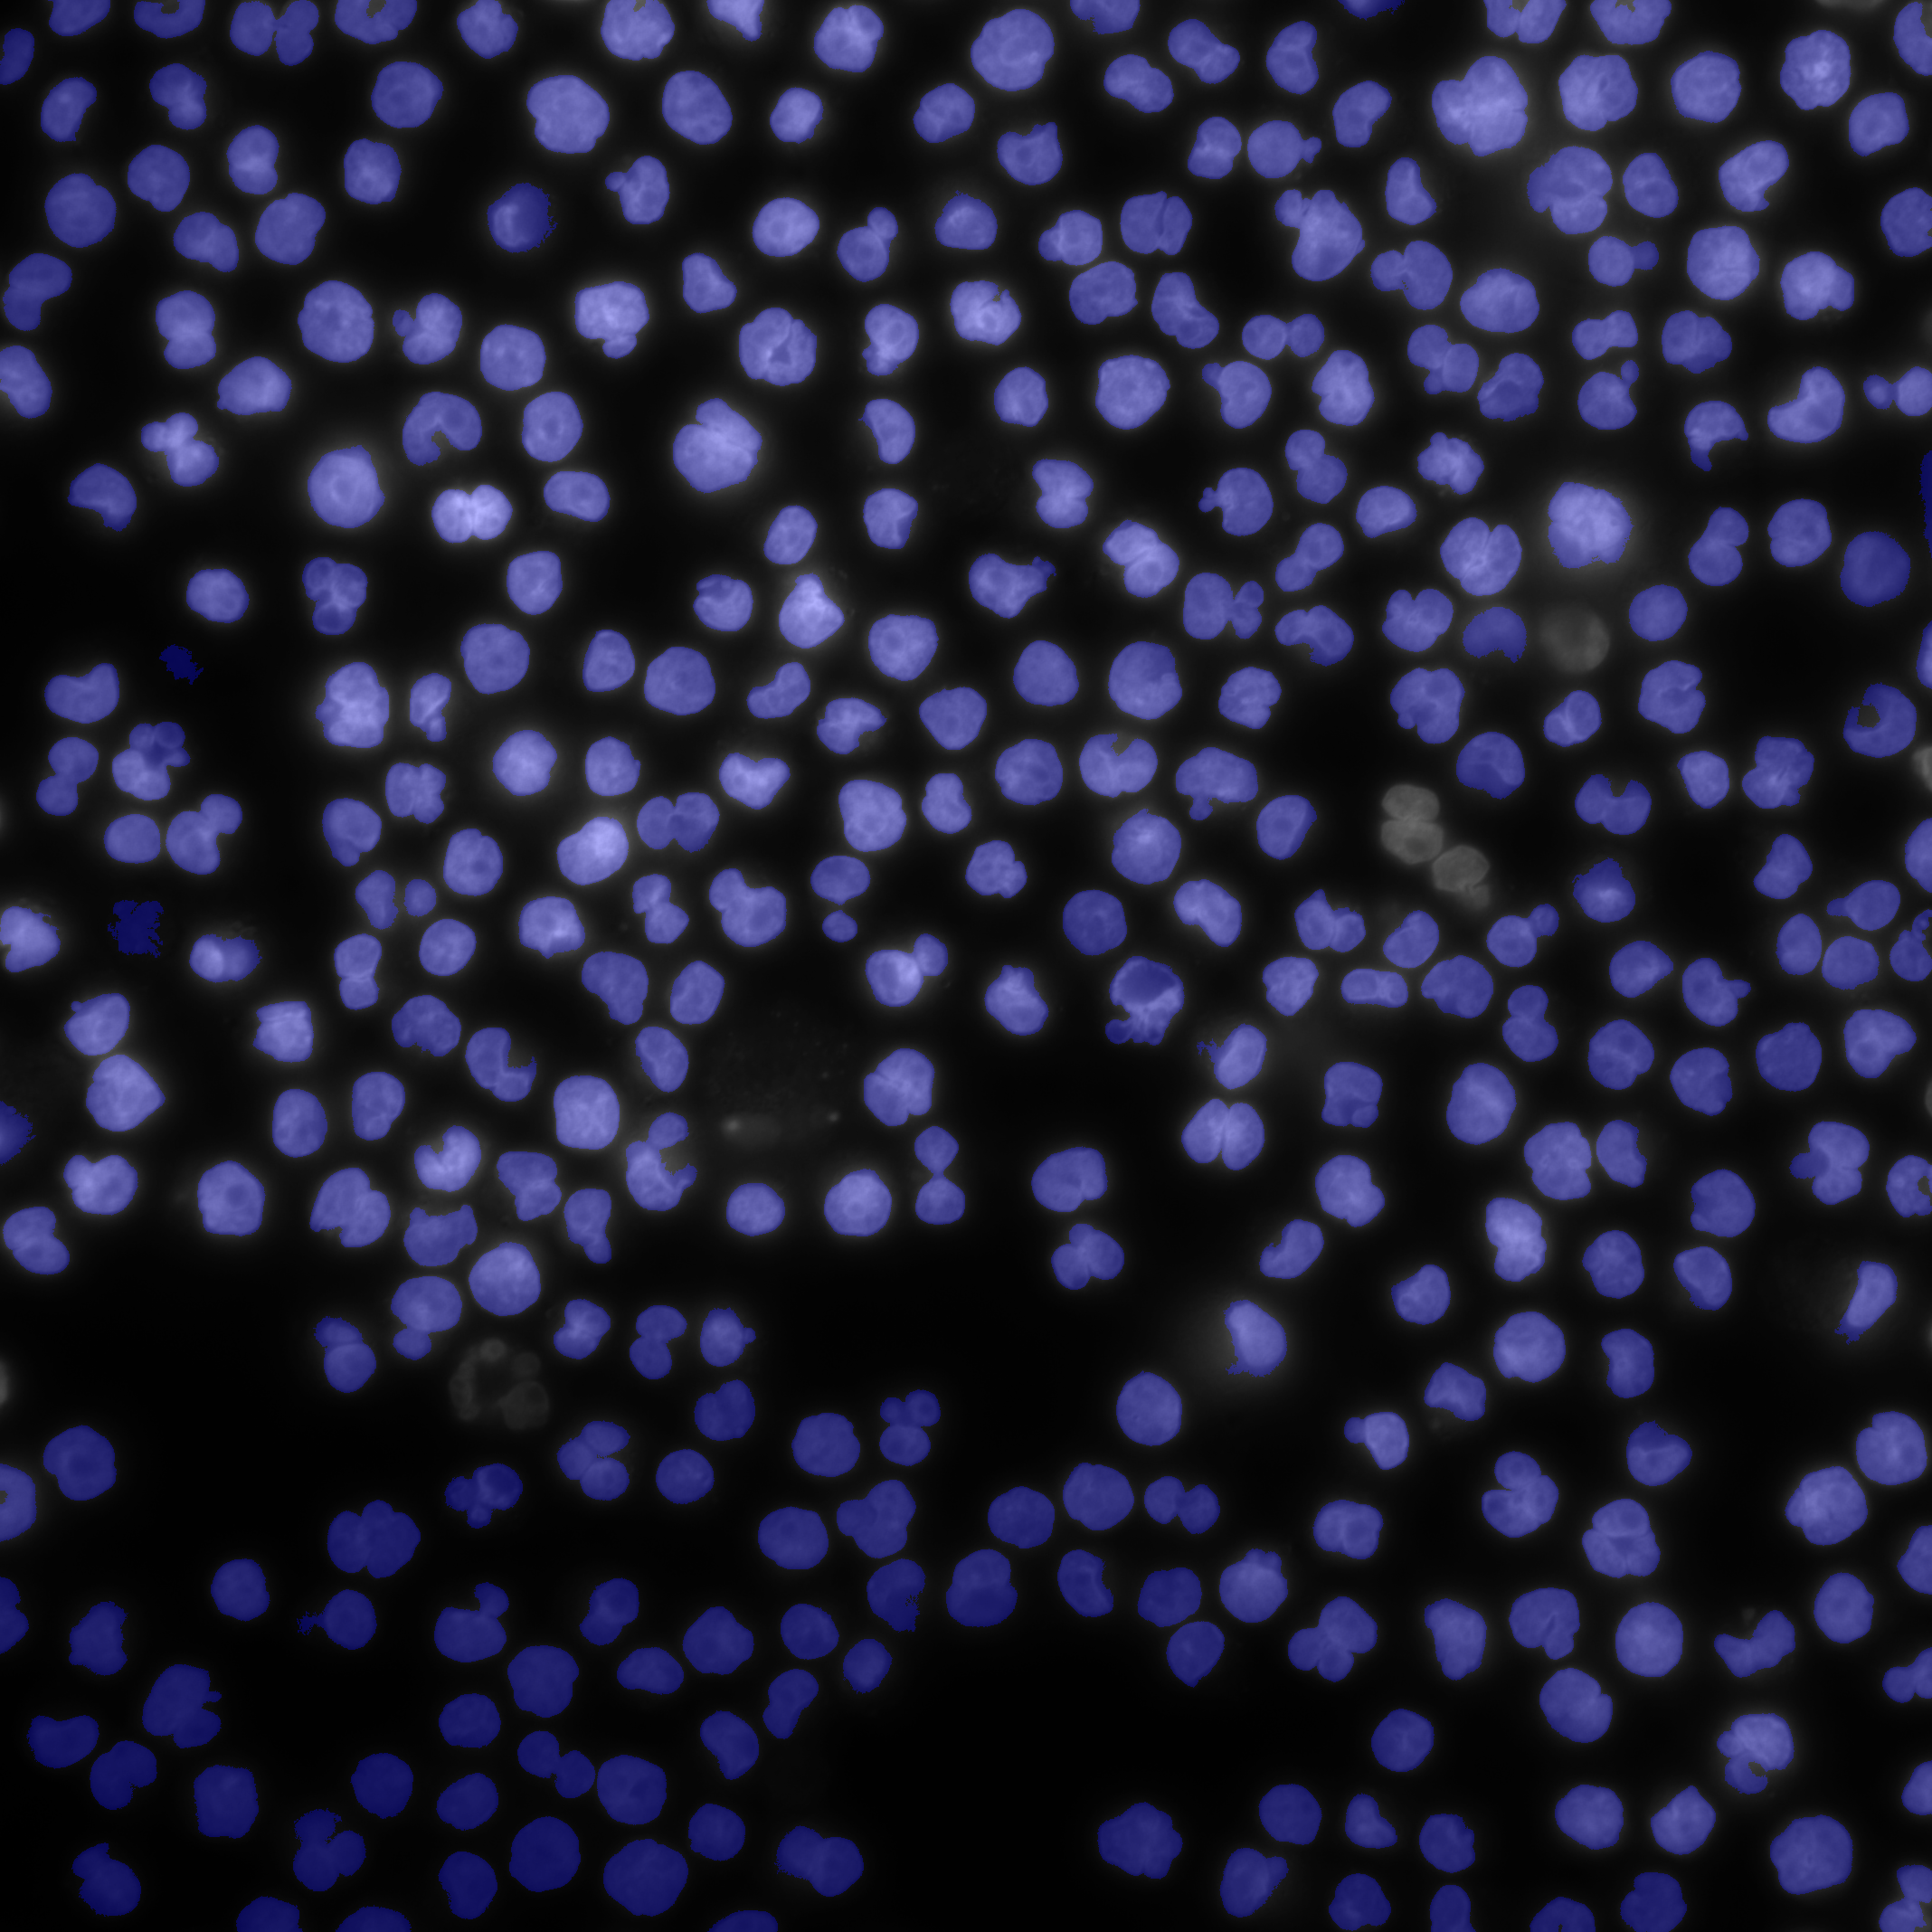
\includegraphics[width=0.75\linewidth]{bilder/difficult-lightning/gradient_local.png} 
      \caption{Local} 
      \label{fig7:a} 
      \vspace{4ex}
    \end{subfigure}%% 
    \begin{subfigure}[b]{0.5\linewidth}
      \centering
      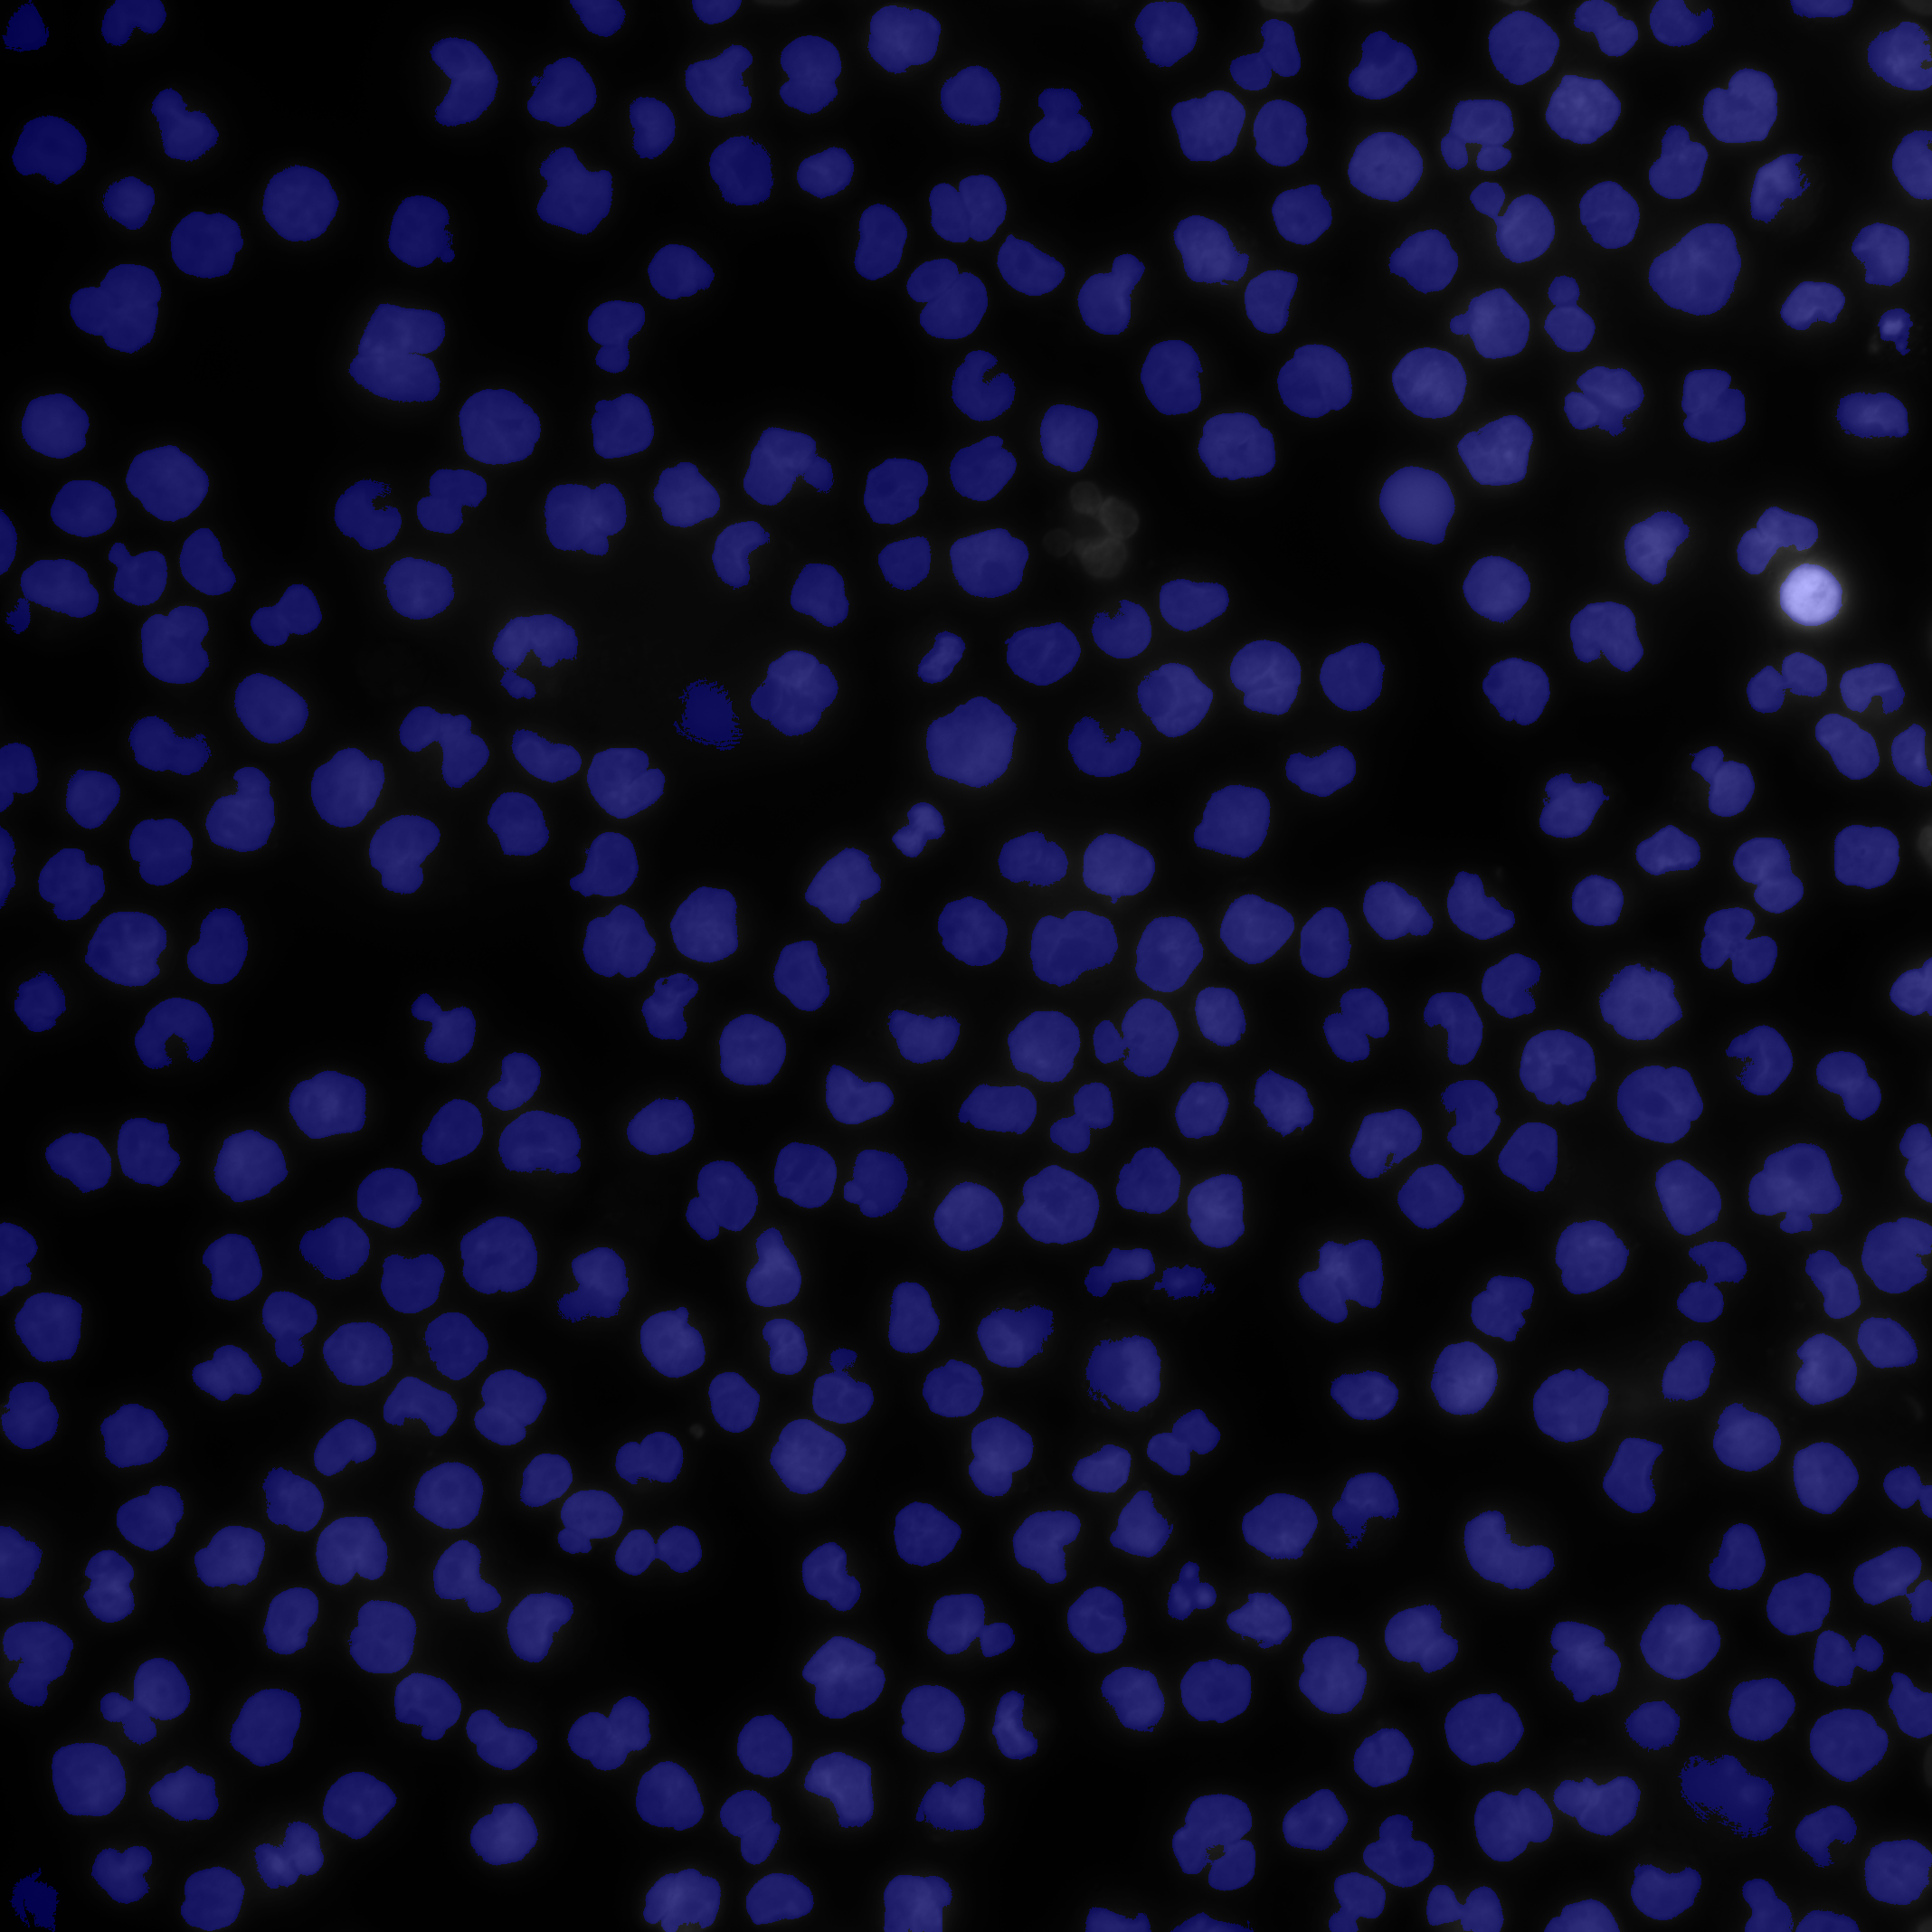
\includegraphics[width=0.75\linewidth]{bilder/difficult-lightning/point_local.png} 
      \caption{Local} 
      \label{fig7:b} 
      \vspace{4ex}
    \end{subfigure} 
    \begin{subfigure}[b]{0.5\linewidth}
      \centering
      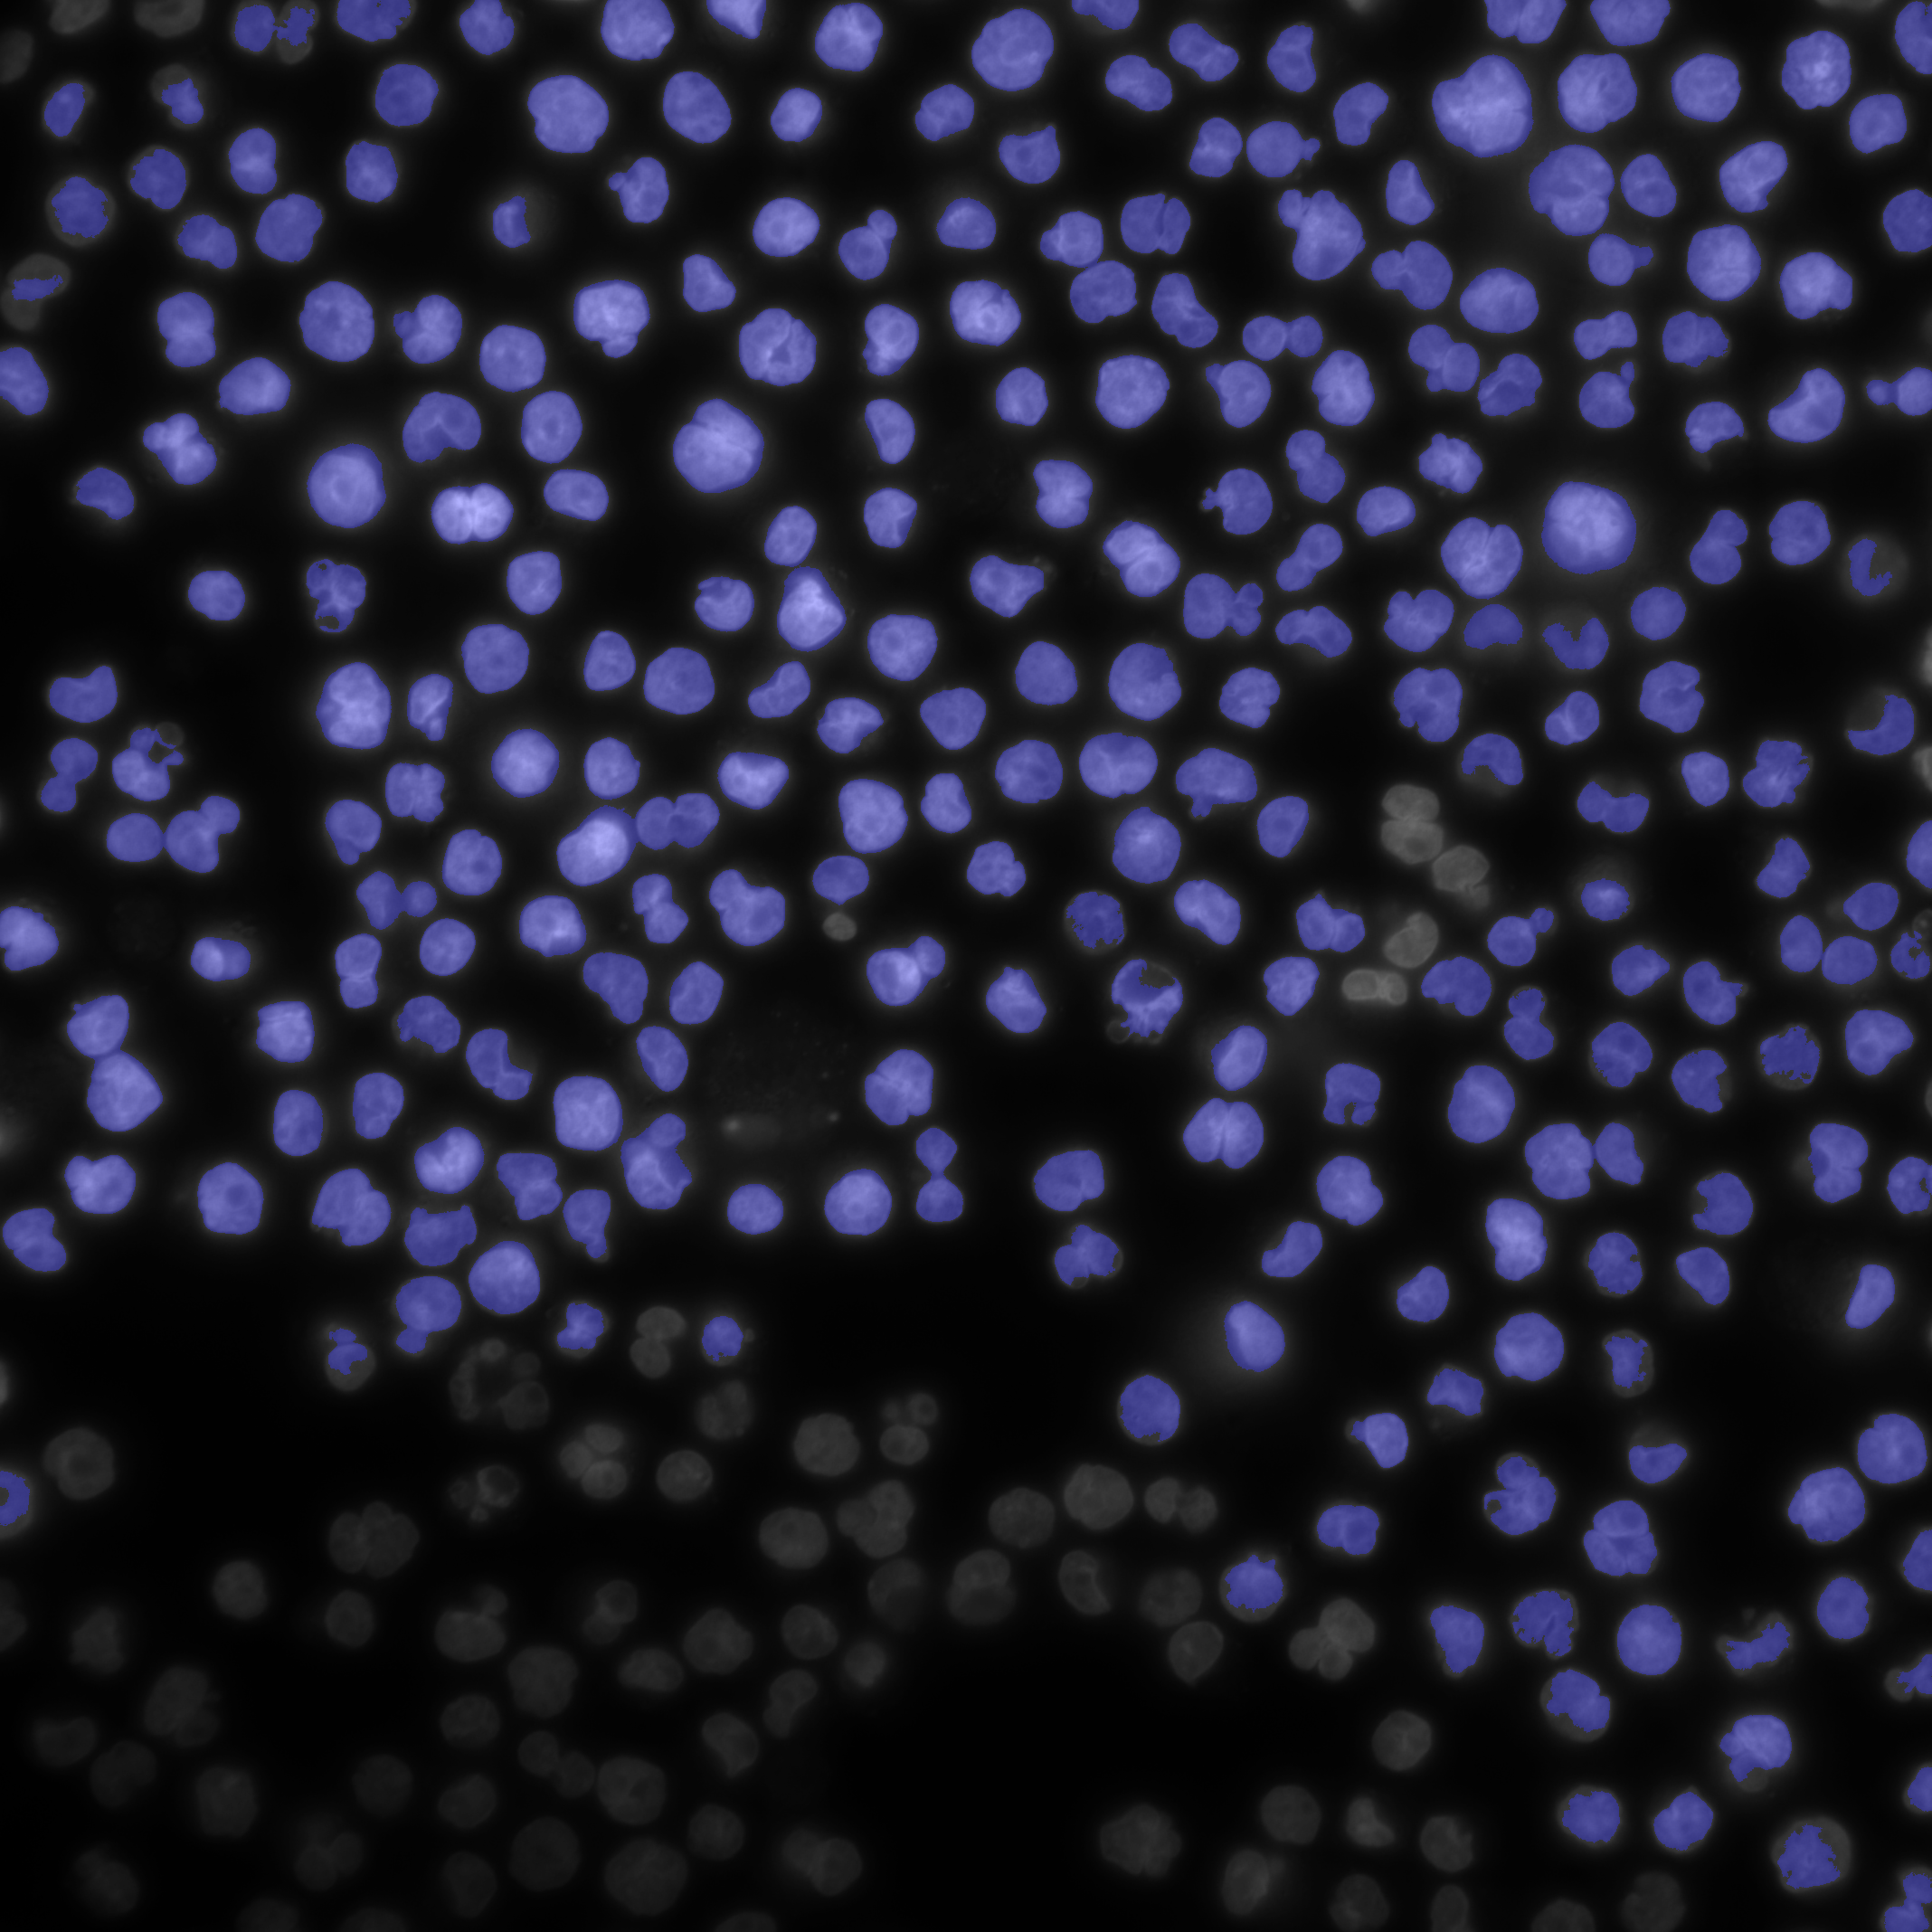
\includegraphics[width=0.75\linewidth]{bilder/difficult-lightning/gradient_min.png} 
      \caption{Global, minimum} 
      \label{fig7:c} 
    \end{subfigure}%%
    \begin{subfigure}[b]{0.5\linewidth}
      \centering
      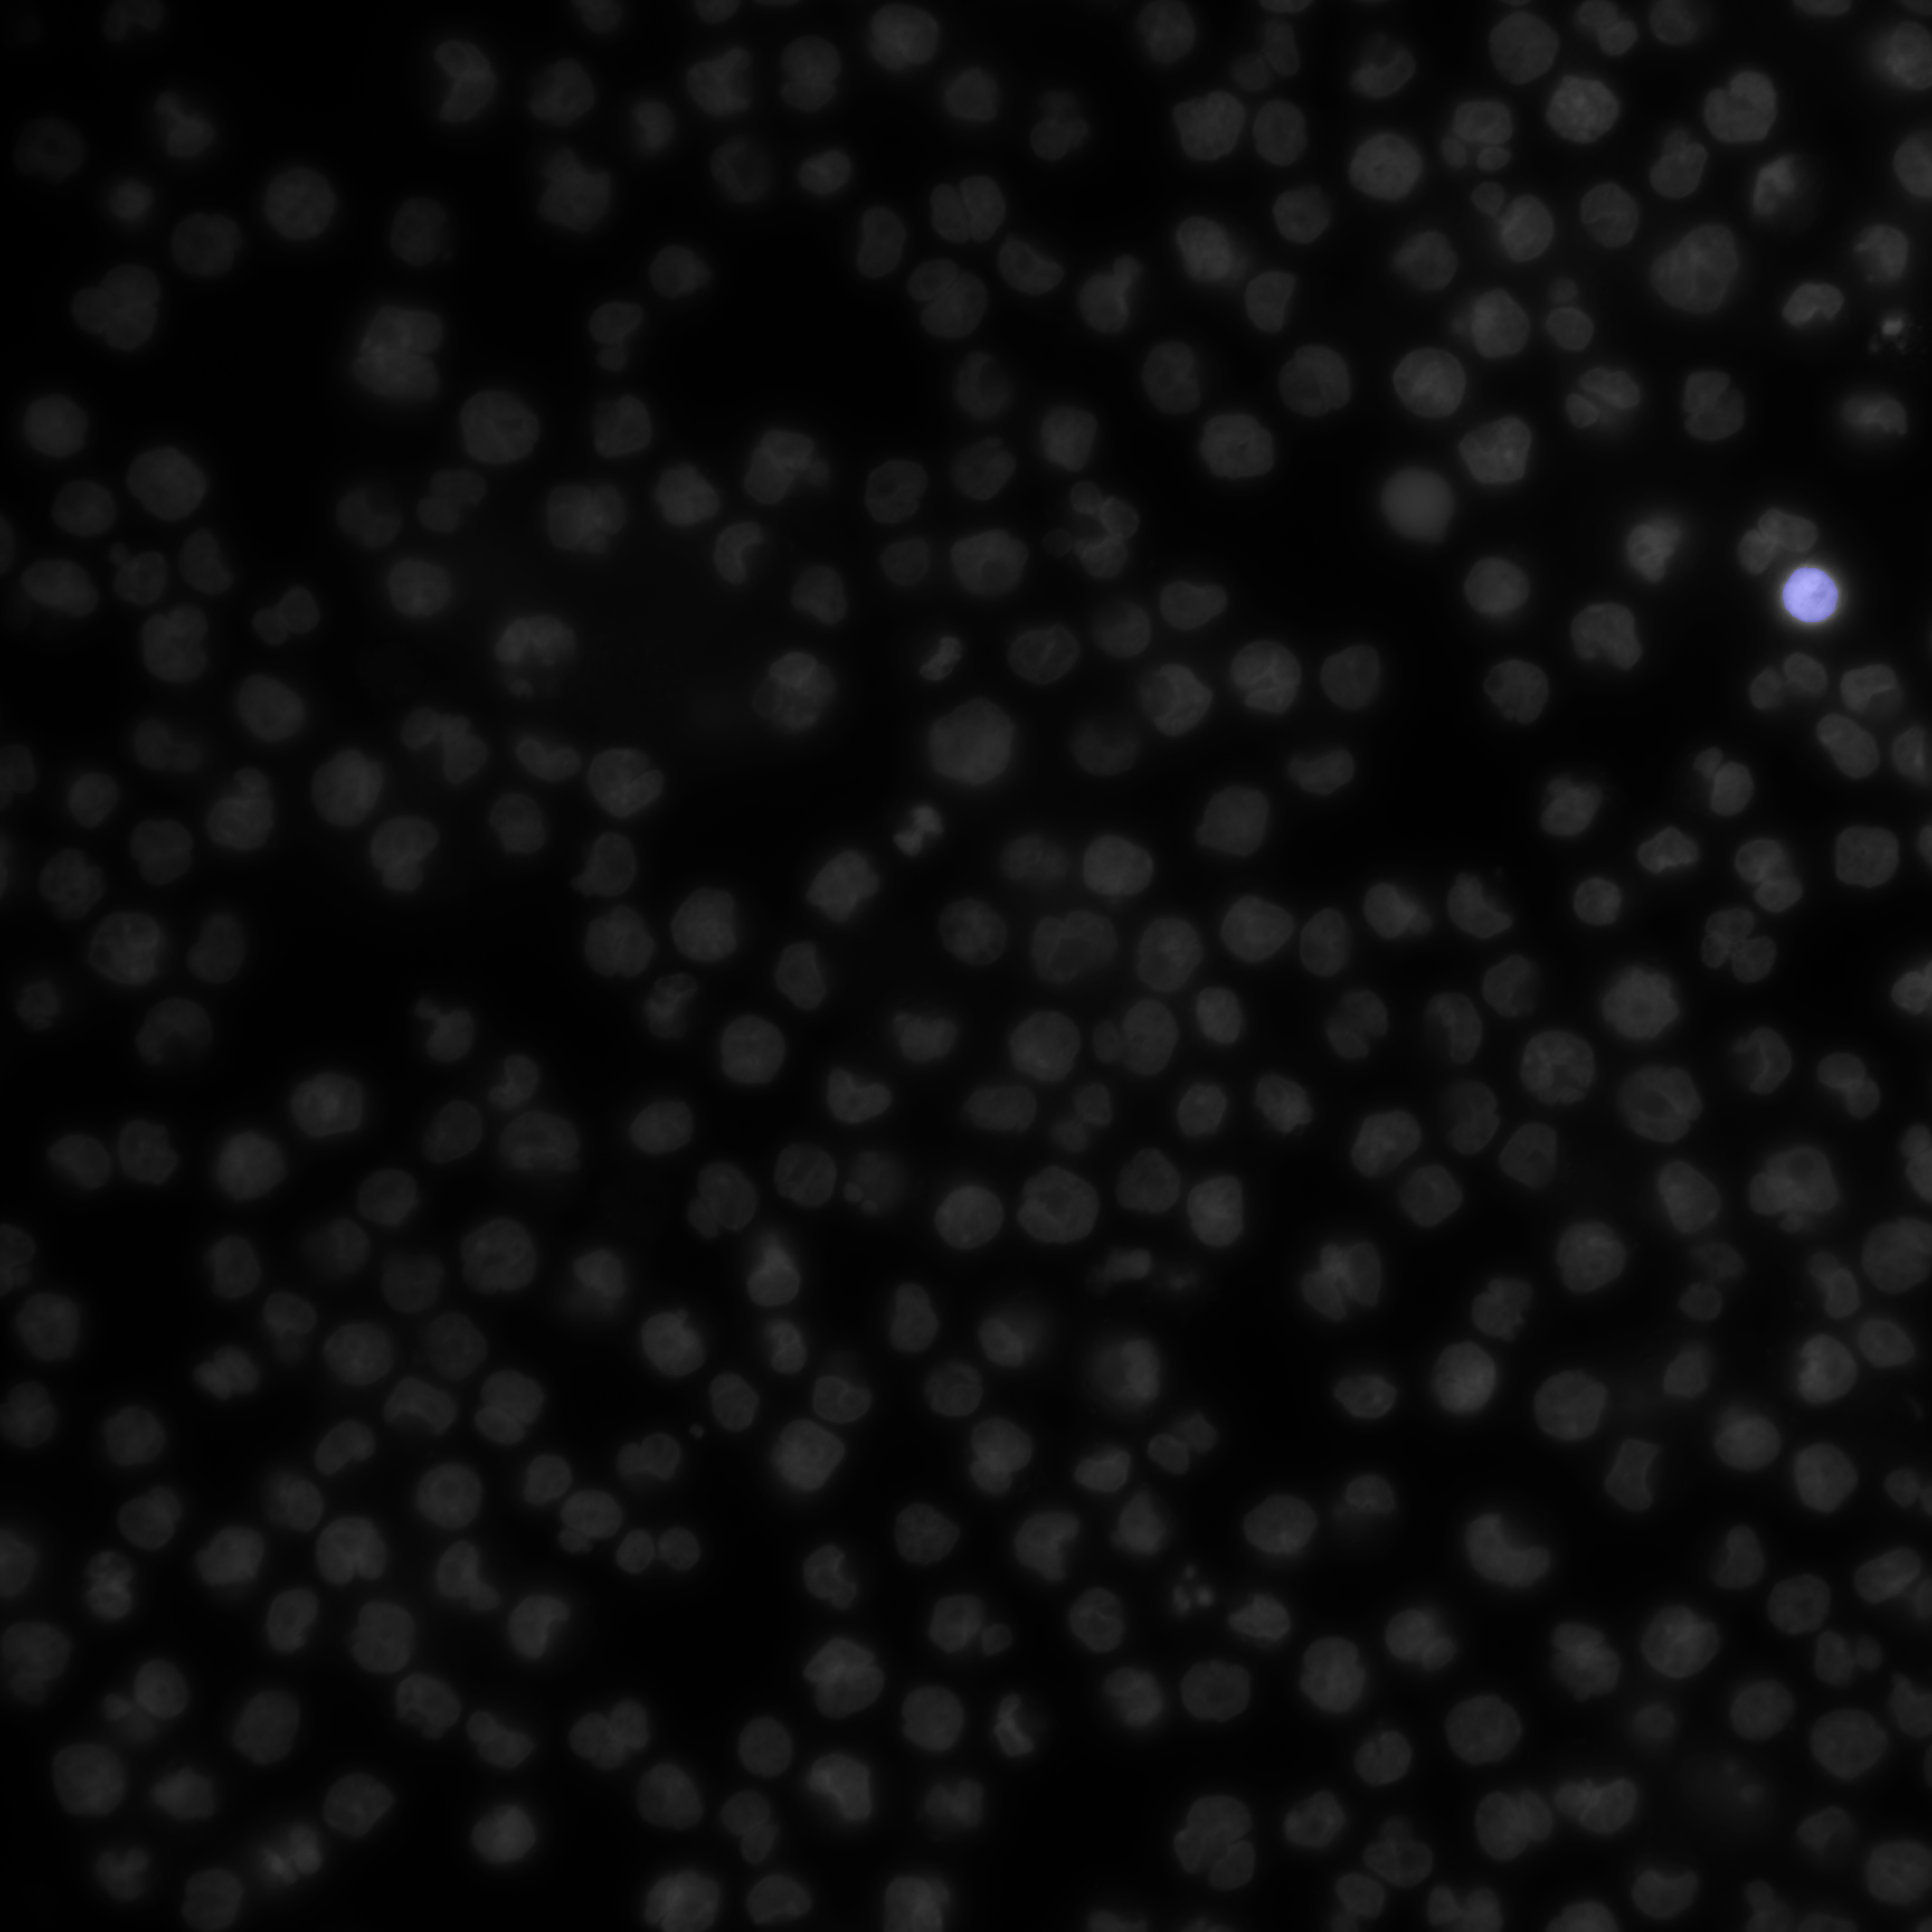
\includegraphics[width=0.75\linewidth]{bilder/difficult-lightning/point_min.png} 
      \caption{Global, minimum} 
      \label{fig7:d} 
    \end{subfigure} 
    \caption{Local vs. Global thresholding}
    \label{fig7} 
\end{figure}

\begin{figure}[H]
    \centering
    \setkeys{Gin}{width=\linewidth}
    \centering
        \begin{tabularx}{\textwidth}{YY}
            \textbf{Local thresholding} &
            \textbf{Minimum thresholding} \\
            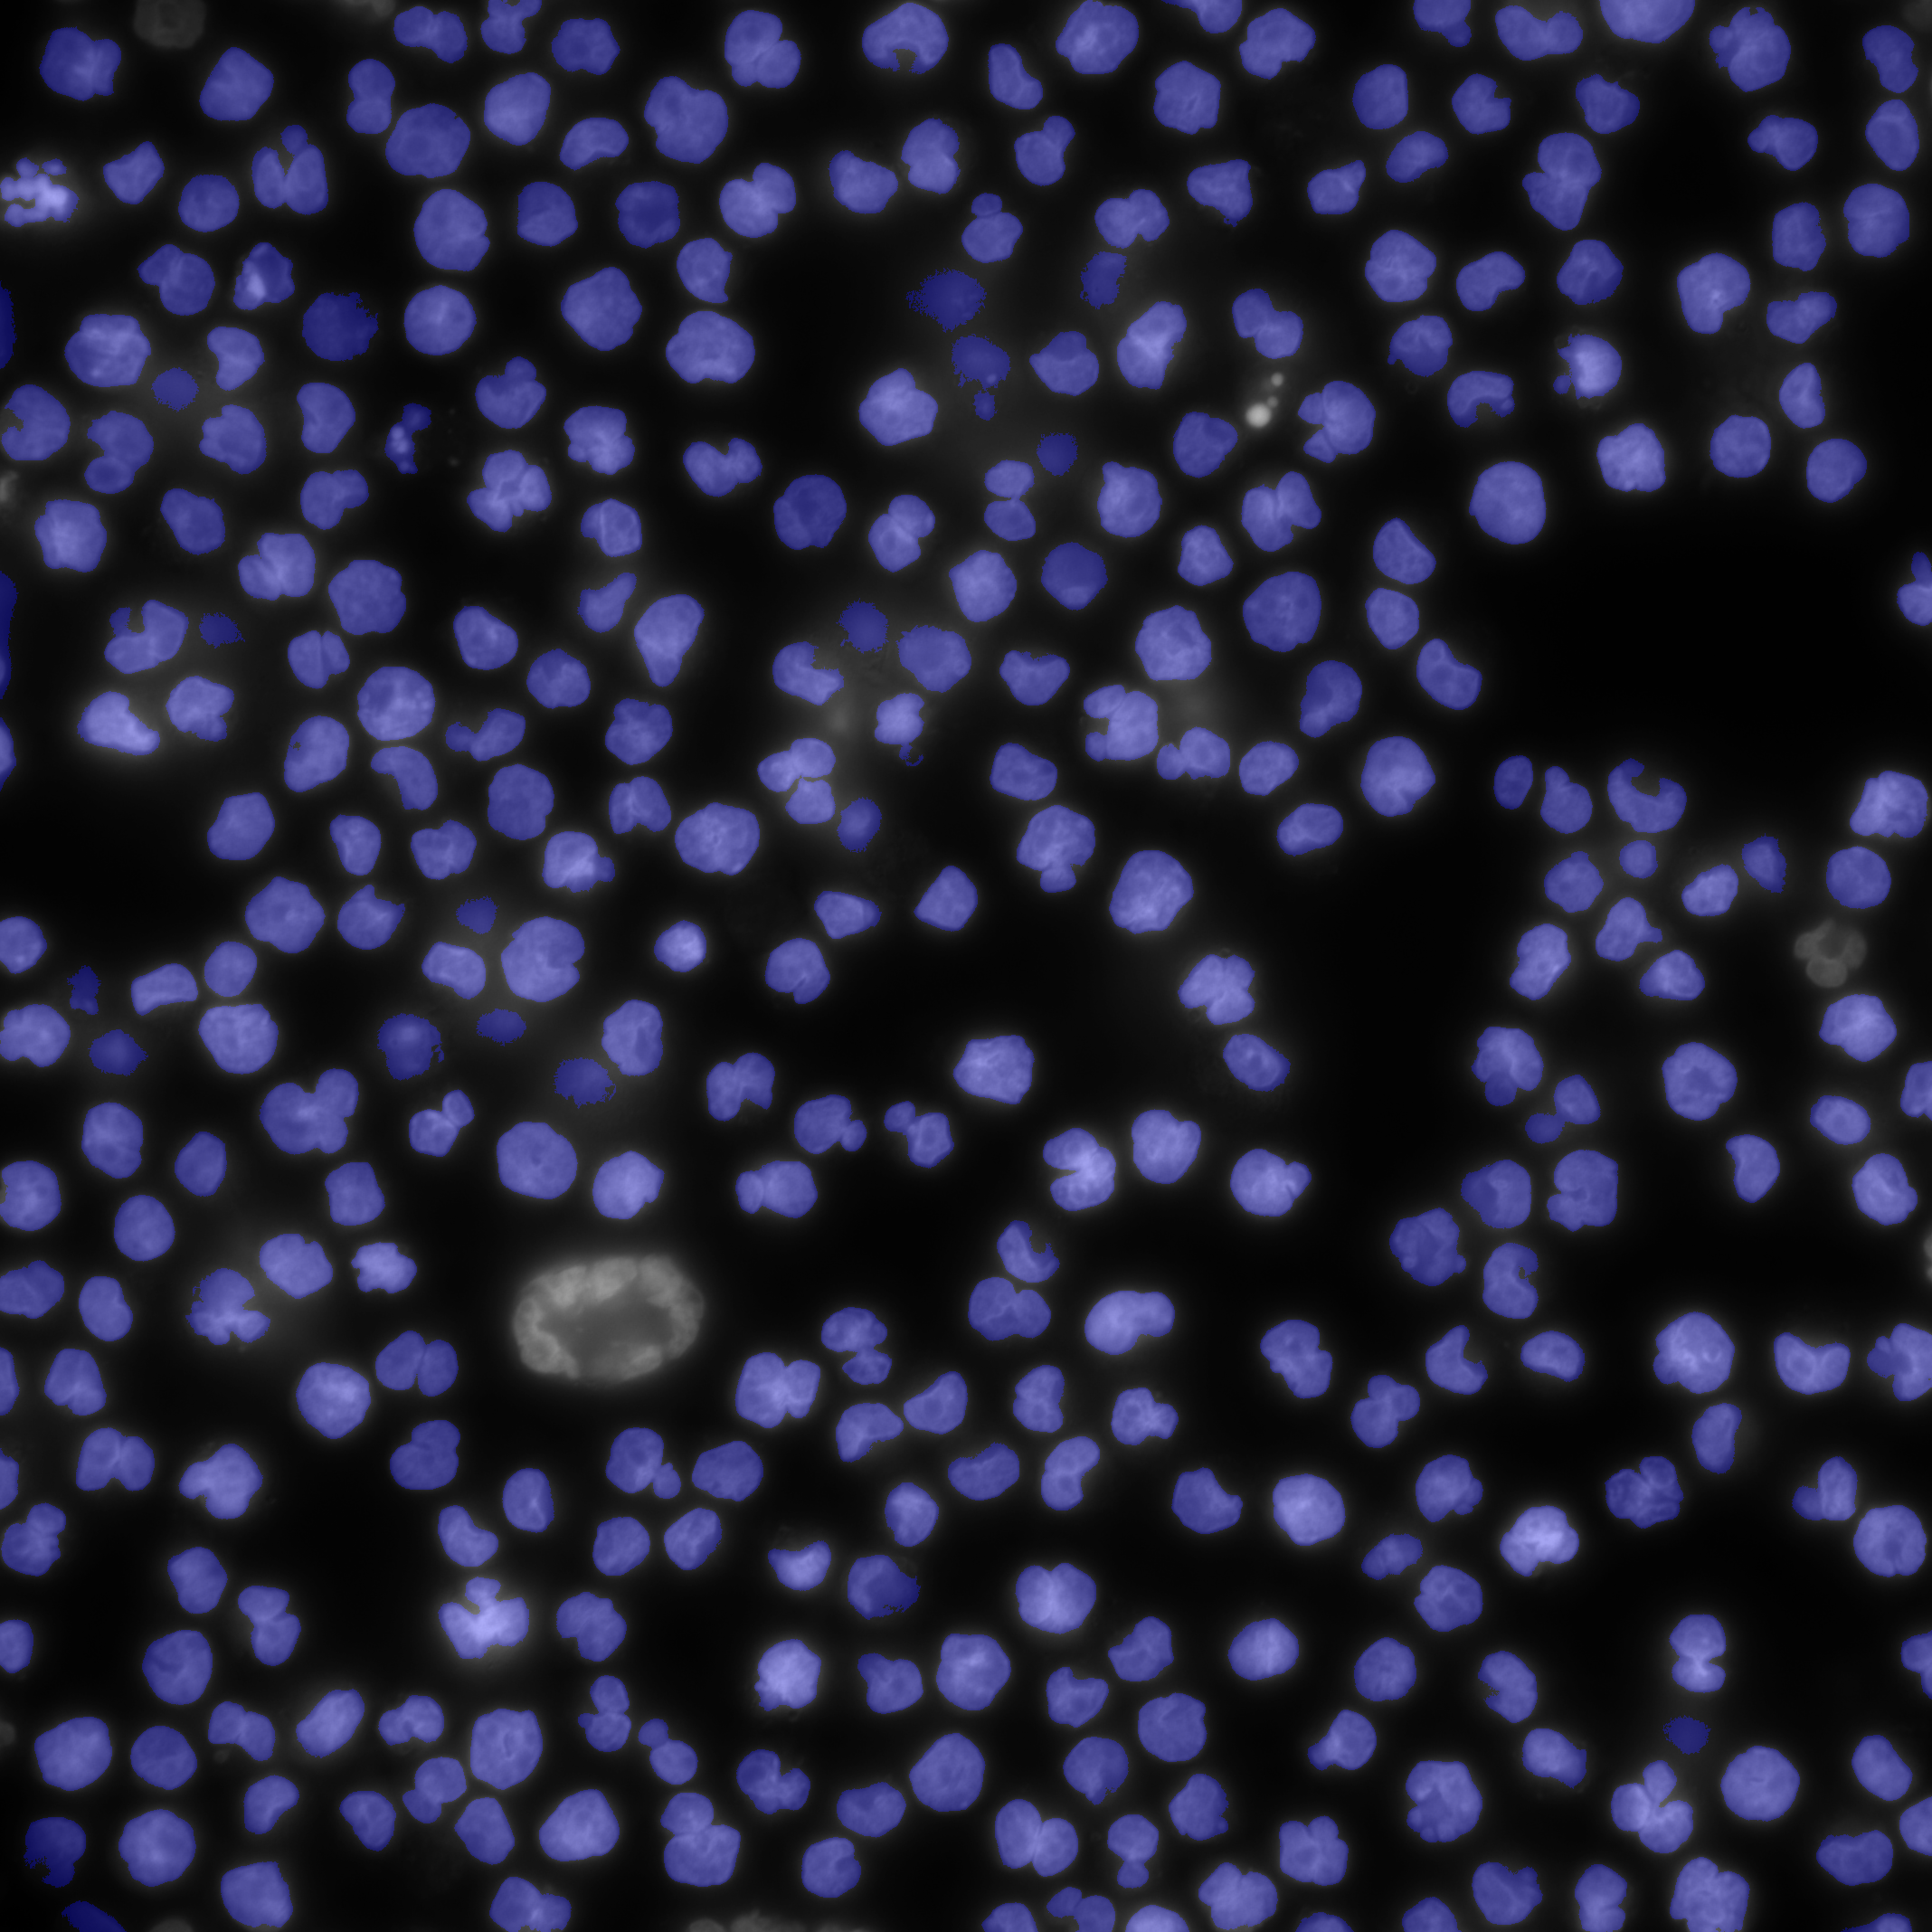
\includegraphics{bilder/difficult-lightning/normal_local.png} & 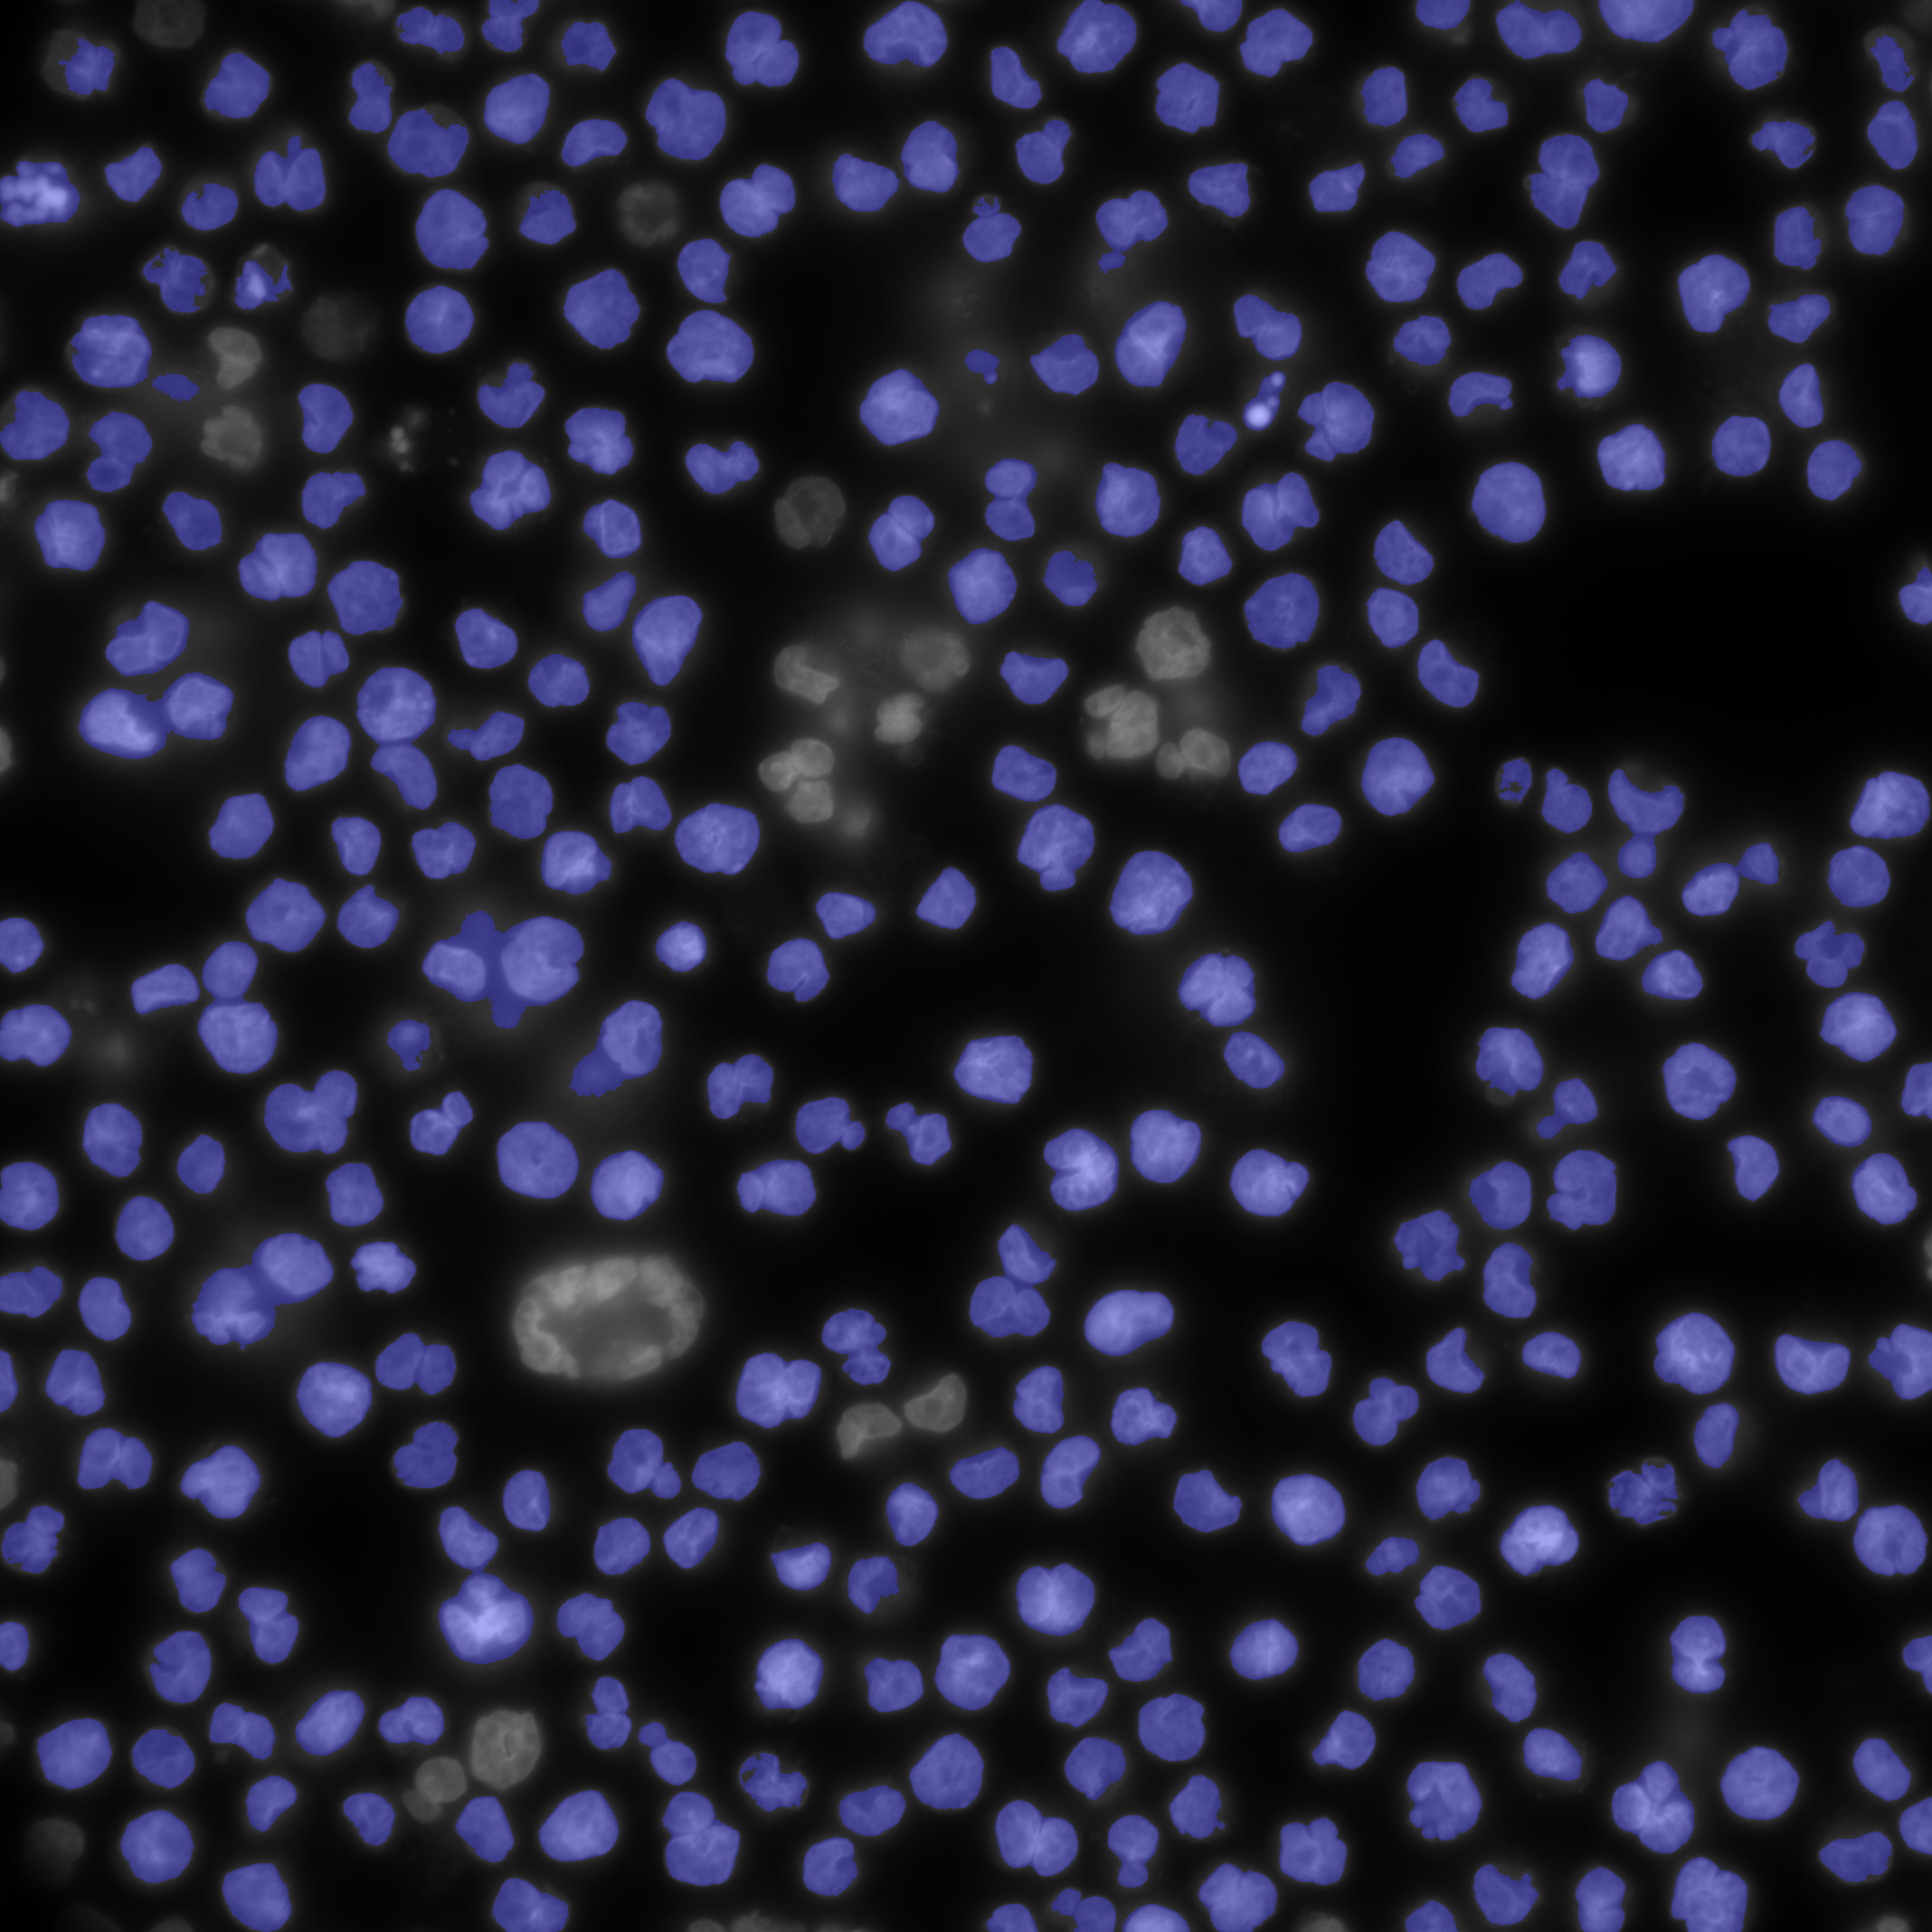
\includegraphics{bilder/difficult-lightning/normal_min.png}
        \end{tabularx}
    \caption{Local vs. Global thresholding (normal conditions)}
    \label{fig:local-vs-global-normal}
\end{figure}
